\documentclass[12pt]{article}                         
\pagestyle{plain}

\usepackage{latexsym}
\usepackage{amssymb}
\usepackage{amsfonts}
\usepackage{amstext}
\usepackage{multicol}
\usepackage{graphicx}
\usepackage{geometry}
\usepackage{tikz}
\usepackage{xcolor} 
\usepackage{textcomp}
\usepackage{pgfplots}
\usepackage{circledtext}
\usepackage{amsmath}
\usepackage{comment}
\usepackage{enumerate}
\usepackage{tabularx} % Used for full-width tables
\usepackage{array}    % Needed for \newcolumntype
\geometry{a4paper, margin=1in}

\begin{document}  

\begin{comment}
\noindent
ALL UNIQUE SLOPES (Total: 10 pairs)
\\
$[-13.0, -4.0, -2.0, -1.0,  0.0, $
$   2.0,  3.0,  5.0, 7.0, 20.0]$

\noindent
\begin{tabular}{ |c|c|c|c|c|c|c|c|c|c| } 
 \hline
 -13 & -4 & -2 & -1 & 0 & 2 & 3 & 5 & 7 & 20 \\
 \hline
 A & B & C & D & E & F & G & H & I & J  \\ 
 \hline
\end{tabular}     
\\
\noindent
POINTS: $(0,15),(3,9),(-3,9),(-4,-5),(2,-11)$\\
KEY: I\_LIKE\_BONUS\_POINTS
\end{comment}
\section*{ACTIVITY}
\begin{center}   
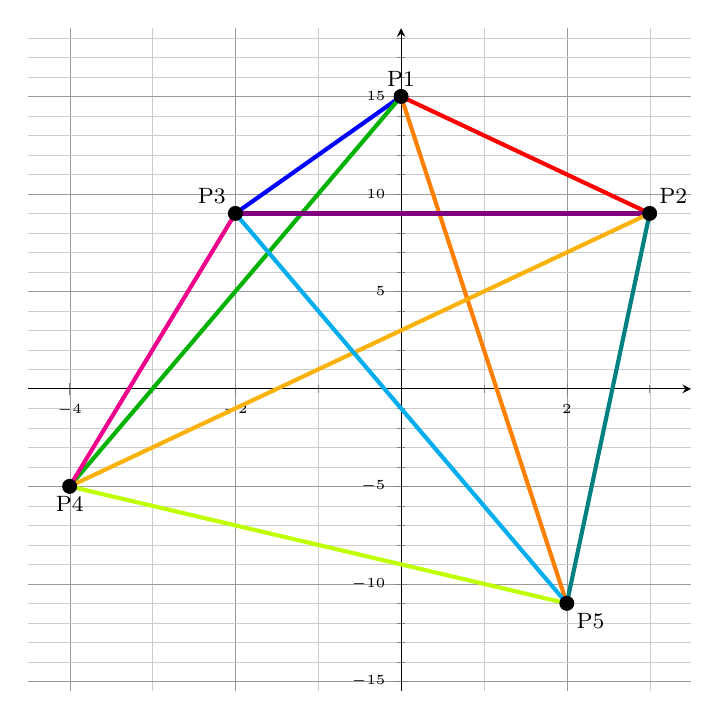
\begin{tikzpicture}
\begin{axis}[
    % Set the overall dimensions of the plot area
    height=10cm, 
    width=10cm,  
    % Set the domain and range for the axes
    xmin=-4.5, xmax=3.5,
    ymin=-15.5, ymax=18.5,
    % Manually set the tick marks
    xtick={-4,-2,0,2,4},
    ytick={-15,-10,-5,0,5,10,15,20},
    % Add 5 minor lines between each major tick on both axes
    minor x tick num=1,
    minor y tick num=4,
    % This command draws both major and minor grid lines
    grid=both,
    major grid style={line width=.1pt,draw=gray!80},
    minor grid style={line width=.1pt,draw=gray!40},
    % Axis and label styling
    axis lines=middle,
    tick label style={font=\tiny},
    xlabel style={at={(current axis.right of origin)}, anchor=west},
    ylabel style={at={(current axis.above origin)}, anchor=south},
    axis line style={-stealth}
]

% --- LINES STARTING AT P1 (0, 15) ---
% 1. P1 to P2
\draw[line width=1.5pt, draw=red]      (axis cs:0,15) -- (axis cs:3,9);
% 2. P1 to P3
\draw[line width=1.5pt, draw=blue]     (axis cs:0,15) -- (axis cs:-2,9);
% 3. P1 to P4
\draw[line width=1.5pt, draw=green!70!black] (axis cs:0,15) -- (axis cs:-4,-5);
% 4. P1 to P5
\draw[line width=1.5pt, draw=orange]   (axis cs:0,15) -- (axis cs:2,-11);

% --- LINES STARTING AT P2 (3, 9) ---
% 5. P2 to P3
\draw[line width=1.5pt, draw=violet]   (axis cs:3,9) -- (axis cs:-2,9);
% 6. P2 to P4
\draw[line width=1.5pt, draw=yellow!70!red] (axis cs:3,9) -- (axis cs:-4,-5); % Gold/Ochre
% 7. P2 to P5
\draw[line width=1.5pt, draw=teal]     (axis cs:3,9) -- (axis cs:2,-11);

% --- LINES STARTING AT P3 (-2, 9) ---
% 8. P3 to P4
\draw[line width=1.5pt, draw=magenta]  (axis cs:-2,9) -- (axis cs:-4,-5);
% 9. P3 to P5
\draw[line width=1.5pt, draw=cyan]     (axis cs:-2,9) -- (axis cs:2,-11);

% --- LINE STARTING AT P4 (-4, -5) ---
% 10. P4 to P5
\draw[line width=1.5pt, draw=lime]     (axis cs:-4,-5) -- (axis cs:2,-11);

% --- 2. PLOT ALL 5 POINTS (Markers) ---
\addplot[only marks, mark=*, black, mark size=2.5pt] 
    coordinates {
        (0,15)
        (3,9)
        (-2,9)
        (-4,-5)
        (2,-11)
    };

% --- 3. ADD LABELS (P1, P2, P3, P4, P5) ---
% Labels are positioned slightly above/below the points for clarity.
\node[above, font=\footnotesize] at (axis cs:0,15) {P1};
\node[above right, font=\footnotesize] at (axis cs:3,9) {P2};
\node[above left, font=\footnotesize] at (axis cs:-2,9) {P3};
\node[below, font=\footnotesize] at (axis cs:-4,-5) {P4};
\node[below right, font=\footnotesize] at (axis cs:2,-11) {P5};

\end{axis}
\end{tikzpicture}
\end{center}

\newcolumntype{W}{>{\centering\arraybackslash}p{0.7cm}} 
\section*{Slope value to Letter table}
% --- Table 1: Columns 1-14 (14 columns) ---
\noindent % Prevents indentation before the table
\begin{tabularx}{\textwidth}{|*{14}{W|}} % 14 Left-aligned (L) columns
\hline
\textbf{-20} & \textbf{-18} & \textbf{-16} & \textbf{-13} & \textbf{-11} & \textbf{-10} & \textbf{-7} & \textbf{-6} & \textbf{-5} & \textbf{-4} & \textbf{-3} & \textbf{-2} & \textbf{-1} & \textbf{0} \\
\hline
J & R & Y & C & S & D & Q & G & T & A & K & N & I & \_ \\
\hline
\end{tabularx}

\vspace{1em} % Add vertical space between tables

% --- Table 2: Columns 15-28 (14 columns) ---
\noindent
\begin{tabularx}{\textwidth}{|*{14}{W|}} % 14 Left-aligned (L) columns
\hline
\textbf{1} & \textbf{2} & \textbf{3} & \textbf{4} & \textbf{5} & \textbf{6} & \textbf{7} & \textbf{10} & \textbf{11} & \textbf{13} & \textbf{16} & \textbf{18} & \textbf{20} & \textbf{---} \\
\hline
U & H & V & W & O & L & E & B & M & F & P & Z & ? & --- \\
\hline
\end{tabularx}

\section*{Write out the solution}


% Optional: A simpler, non-grid version for pure console display:
% \vspace{1cm}
\newcolumntype{W}{>{\centering\arraybackslash}p{0.7cm}} 

\noindent \rule{0.3cm}{0.4pt} \rule{0.3cm}{0.4pt} \rule{0.3cm}{0.4pt} \quad \rule{0.3cm}{0.4pt} \quad \rule{0.3cm}{0.4pt} \rule{0.3cm}{0.4pt} \rule{0.3cm}{0.4pt} \rule{0.3cm}{0.4pt} \quad \rule{0.3cm}{0.4pt} \rule{0.3cm}{0.4pt} \rule{0.3cm}{0.4pt} \rule{0.3cm}{0.4pt} \rule{0.3cm}{0.4pt} \quad \rule{0.3cm}{0.4pt} \rule{0.3cm}{0.4pt} \rule{0.3cm}{0.4pt} \rule{0.3cm}{0.4pt} \rule{0.3cm}{0.4pt} \rule{0.3cm}{0.4pt} \quad ?
\\\\
\noindent % Prevents indentation before the table
\begin{tabularx}{\textwidth}{|*{14}{W|}} % 14 Left-aligned (L) columns
\hline
& & & & & & & & & & & & \\
\hline
C & A & N & \_ & I & \_ & H & A & V & E & \_ & T & W & O \\
\hline
\end{tabularx}

\vspace{1em} % Add vertical space between tables

% --- Table 2: Columns 15-28 (14 columns) ---
\noindent
\begin{tabular}{|*{13}{W|}} 
\hline
\multicolumn{13}{|c|}{\textbf{BONUS POINTS ?}} \\
\hline
% ROW 2: Letters - 13 Items exactly. The space is omitted for brevity.
\textbf{B} & \textbf{O} & \textbf{N} & \textbf{U} & \textbf{S} & \textbf{P} & \textbf{O} & \textbf{I} & \textbf{N} & \textbf{T} & \textbf{S} & \textbf{?} & \textbf{\_} \\
\hline
\end{tabular}

\end{document}